
Above we reviewed some existing classification methods for security metrics. These included taxonomies from both narrow and broadly focused surveys. While there is certainly overlap within some of the categories and properties identified, there is also collision between similar sounding concepts from different sources. To remove ambiguity, and more importantly to address the immediate question, we can map all our security metrics onto the taxonomy derived from the Cyber Security Body of Knowledge. The CyBoK is an effort to collect and maintain canonical research across the entirety of the cyber security domain. Included in this mandate is keeping all of it organized, so we can presume that if there is a topic in security we would like to measure, then there will be a corresponding topic in the CyBoK to consult. 

Security metrics can be categorized by the area of cyber security to which they apply. In this respect, the security metric surveys available in recent literature are by nature focused narrowly on a specific subfield, such as cryptographic or software development lifecycle security metrics. To remove ambiguity in terms among surveys, we attempt to include these in a \textit{big-picture} view of the field of cyber security by classifying them under the general headings of the recently released Cyber Security Body of Knowledge\cite{Rashid_Chivers_Danezis_Lupu_Martin} depicted in Figure \ref{fig:intro:cybok}. By grouping our security metrics by Cybok category, we can determine our cyber security metric coverage, and use this context to identify non-security related metrics that would be relevant to the area. 

\subsubsection{Human, Organization, \& Regulatory Metrics}

\begin{figure}[ht]

\begin{mdframed}
\centering
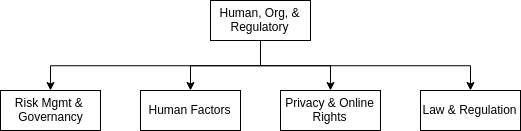
\includegraphics[width=.8\linewidth]{resource/img/ch_background/cybok_metrics/cybok_hor.png}
\end{mdframed}
\caption{Cybok: Human, Organization, \& Regulation Metrics
\label{fig:background:cybok_hor_metrics}}
\end{figure} 

\begin{figure}[ht]
\centering
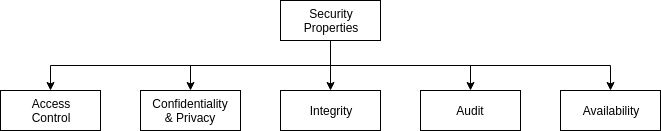
\includegraphics[width=.9\linewidth]{resource/img/ch_background/cybok_metrics/morrison_sec_props.png}
\caption{Most of Morrison’s class for Security Properties would fit under HO\&R.
\label{fig:background:cybok_hor_metrics_morrison}}
\end{figure} 

\begin{figure}[ht]
\centering
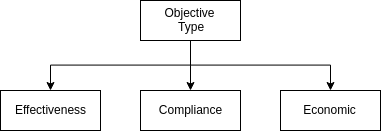
\includegraphics[width=.6\linewidth]{resource/img/ch_background/cybok_metrics/ramos_objective_type.png}
\caption{Ramos’ Objective Type metrics fall under HO\&R (economics is cross cutting).
\label{fig:background:cybok_hor_metrics_ramos}}
\end{figure} 


\begin{figure}[ht]
\centering
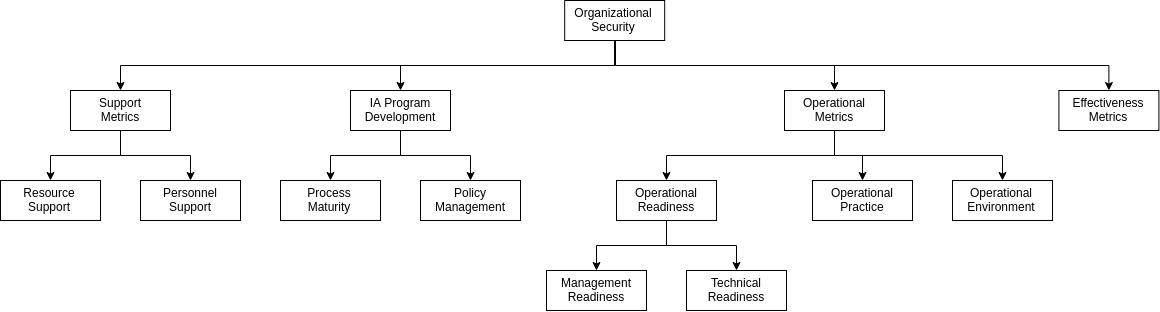
\includegraphics[width=.95\linewidth]{resource/img/ch_background/cybok_metrics/vaughn_org_metrics.png}
\caption{Vaughn’s Organization Security metrics subtree  falls under HO\&R.
\label{fig:background:cybok_hor_metrics_vaughn}}
\end{figure} 

Metrics in HO\&R are usually derived from applicable regulations and policies (ISO, FISMA, HIPPA, PCI, ADA, etc). Often these are counts or ratios that quantify the proportion of assets that are in/out of compliance with the regulation. Typical applications for these metrics are system audits (how many current users have completed mandatory training) or accreditations (how many of these secure operations checkboxes does the current system check).


\subsubsection{Attack \& Defense Metrics}

\begin{figure}[ht]

\begin{mdframed}
\centering
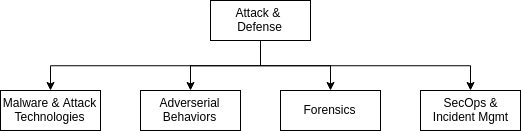
\includegraphics[width=.8\linewidth]{resource/img/ch_background/cybok_metrics/cybok_ad.png}
\end{mdframed}
\caption{Cybok: Attack \& Defense Domain Metrics
\label{fig:background:cybok_ad_metrics}}
\end{figure} 

Attack and defense describes many of the security metrics we have investigated in this thesis. Malware and Attack metrics can quantify an attacker’s capabilities, the DoS’ing bandwidth of a botnet or the number of accounts controlled are examples. Adversarial behaviours might relate to MITRE’s APT and CAPEC attack pattern datasets, but I haven’t encountered metrics that evaluate this yet (although it shows up regularly in threat models). Forensics metrics typically include time to unpack or deobfuscate a malware sample, or the amount of time to determine an indicator of compromise for IDS deployment. SecOps \& Incident Response metrics include standards from the literature such as IDS efficacy and mean time between failures. 

\begin{figure}[ht]
\centering
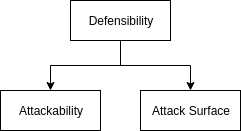
\includegraphics[width=.35\linewidth]{resource/img/ch_background/cybok_metrics/morrison_defensibility.png}
\caption{Morrison’s Defensibility metrics fall generally under A\&D.
\label{fig:background:cybok_ad_morrison}}
\end{figure} 

\begin{figure}[ht]
\centering
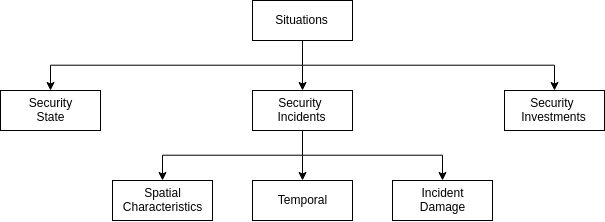
\includegraphics[width=.8\linewidth]{resource/img/ch_background/cybok_metrics/pendleton_situations.png}
\caption{Pendleton’s Situations metrics fall under A\&D.
\label{fig:background:cybok_ad_pendleton}}
\end{figure} 

\begin{figure}[ht]
\centering
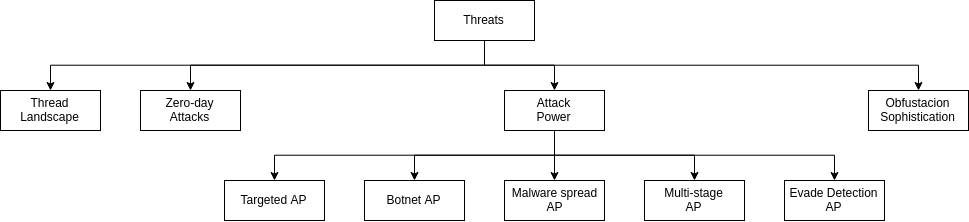
\includegraphics[width=.95\linewidth]{resource/img/ch_background/cybok_metrics/pendleton_threats.png}
\caption{Pendleton’s Threats metrics fall under A\&D.
\label{fig:background:cybok_ad_pendleton_threats}}
\end{figure} 

\begin{figure}[ht]
\centering
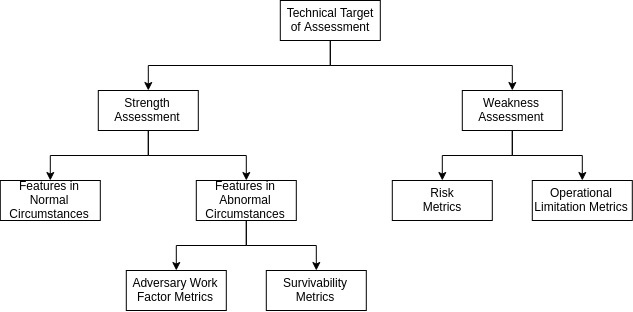
\includegraphics[width=.75\linewidth]{resource/img/ch_background/cybok_metrics/vaughn_ttoa.png}
\caption{Vaughn’s Strength and Weakness metrics fall under A\&D.
\label{fig:background:cybok_ad_vaugh_ttoa}}
\end{figure} 

\subsubsection{Systems Security Metrics}

\begin{figure}[ht]

\begin{mdframed}
\centering
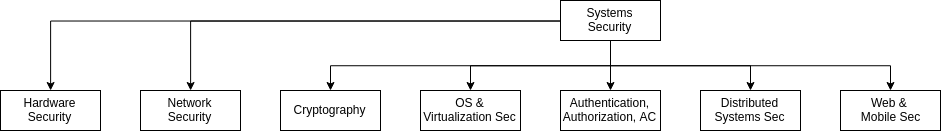
\includegraphics[width=.95\linewidth]{resource/img/ch_background/cybok_metrics/cybok_systems.png}
\end{mdframed}
\caption{Cybok: Systems Domain Metrics
\label{fig:background:cybok_ad_metrics}}
\end{figure} 

Systems security metrics span most aspects of operational security. Hardware and Network security metrics were discussed under infrastructure. Typical applications of cryptographic security metrics include all the formal verification artifacts involved in the validation of a protocol or implementation, along with performance, key size, entropy, etc. OS security metrics may be derived from common criteria/ EAL or measure isolation, weakness to side channels, or number of vulnerabilities known along with severity. 

\begin{figure}[ht]
\centering
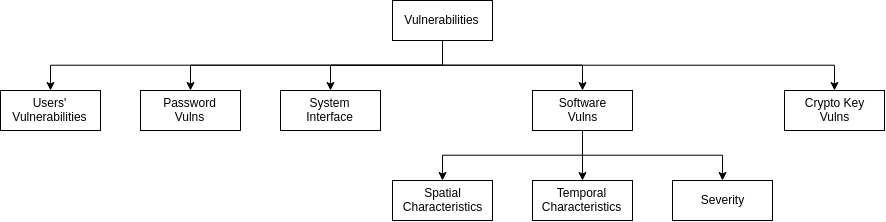
\includegraphics[width=.95\linewidth]{resource/img/ch_background/cybok_metrics/pendleton_vulns.png}
\caption{Pendleton’s Vulnerabilities security metrics fall under System’s security metrics
\label{fig:background:pendleton_vuln_metrics}}
\end{figure} 

Model based network security metrics classified by Ramos\cite{Ramos_Lazar_Filho_Rodrigues_2017} are shown below. These metrics are designated as Compliance based when a larger value indicates more security. Moment identifies if a measurement can be taken pre-deployment and remains static throughout operation, or if the metric is dynamic and should be measured repeatedly. Consistency distinguishes if the measured value relies on subjective human input or if its evaluation is objective. To compare with network performance metrics like latency or throughput, these security metrics are heavily influenced by subjective criteria. For example, the reliability based models make assumptions about an attacker’s success rate, level of effort, motivations, and capabilities that could change depending on who is filling in the weights. 

% \begin{minipage}{\linewidth}
% % \begin{table}[]
% \resizebox{\textwidth}{!}{%
% \begin{tabular}{@{}lllll@{}}
% \toprule
% \textbf{Metric} & \textbf{Compliance} & \textbf{Moment} & \textbf{Consistency} &  \\ \midrule
% MTTF {[}70{]}, {[}71{]} & compliance & dynamic & objective &  \\
% METF {[}72{]} & compliance & dynamic & subjective &  \\
% MTSF {[}40{]}, {[}73{]}, {[}74{]} & compliance & static & subjective &  \\
% MTFF {[}53{]}, {[}54{]} & compliance & static & subjective &  \\
% MTTC by McQueen et al. {[}8{]}, {[}75{]} & compliance & static & subjective &  \\
% MTTC by Leversage et al. {[}76{]} & compliance & static & subjective &  \\
% Steady-State Security {[}40{]}, {[}73{]}, {[}74{]} & non-compliance & static & subjective &  \\
% Reliability {[}79{]} & compliance & static & objective &  \\
% Success Likelihood {[}80{]} & non-compliance & dynamic & subjective &  \\
% q {[}81{]} & non-compliance & static & objective &  \\
% Shortest Path {[}83{]}, {[}10{]} & compliance & dynamic & objective &  \\ 
% Number of Paths {[}72{]}, {[}10{]} & non-compliance & dynamic & objective &  \\
% Mean of Path Lengths {[}95{]}, {[}10{]} & compliance & dynamic & objective &  \\
% Normalized Mean of Path Lengths {[}10{]} & compliance & dynamic & objective &  \\
% Assistive metrics: SDPL, MoPL, MePL {[}10{]} & compliance & dynamic & objective &  \\
% Weakest Adversary {[}96{]}  & compliance & static & subjective&  \\
% Network Compromise Percentage {[}97{]} & non-compliance &  dynamic &  objective &\\
% State Rank {[}98{]} & non-compliance & static & subjective &  \\
% Cumulative Score {[}99{]} & non-compliance & static & objective &  \\
% AGP {[}88{]} & non-compliance & static & subjective &  \\
% Attack Resistance {[}100{]} & compliance & static & subjective &  \\
% Enhanced Cumulative Score {[}102{]} & non-compliance & static & subjective &  \\
% Liu and Man’s metric {[}104{]} & non-compliance & dynamic & subjective &  \\
% Frigault and Wang’s metric {[}105{]} & non-compliance & static & subjective &  \\
% Frigault and colleagues’ metric {[}106{]} & non-compliance & dynamic & subjective &  \\
% Poolsappasit and colleagues’ metric {[}107{]} & non-compliance & dynamic & subjective &  \\
% Xie and colleagues’ metric {[}108{]} & non-compliance & dynamic & subjective &  \\
% Dantu and colleagues’ metric {[}109{]}, {[}110{]}, {[}111{]} & non-compliance & dynamic & subjective &  \\
% Expected Difficulty {[}112{]} & compliance & static & subjective &  \\
% VEA-bility {[}31{]} & compliance & static & subjective &  \\
% k-zero day safety {[}113{]}, {[}114{]} & compliance & static & subjective &  \\
% d2-Diversity (least attacking effort) {[}115{]}, {[}116{]} & compliance & static & subjective &  \\
% d3-Diversity (avg. attacking effort) {[}115{]}, {[}116{]} & non-compliance & static & subjective &  \\
% d1-Diversity (\% of distinct resources) {[}115{]}, {[}116{]} & compliance & static & subjective &  \\
% Seclius {[}118{]} & non-compliance & dynamic & objective &  \\
% Damage risk {[}120{]} & non-compliance & static & subjective &  \\
% Mean Privacy {[}121{]} & non-compliance & static & subjective &  \\
% Security Meter {[}122{]}, {[}123{]} & non-compliance & static & subjective &  \\
% Policy Security Score {[}124{]} & compliance & dynamic & subjective &  \\
% Probabilistic Vulnerability Measure {[}125{]} & non-compliance & dynamic & subjective &  \\
% Attack Propagation {[}126{]} & non-compliance & dynamic & subjective &  \\
% ADVISE {[}127{]} & compliance & static & subjective &  \\ \bottomrule
% \end{tabular}%
% }

% % \caption{Ramos}
% % \label{tab:ramos_metrics}
% % \end{table}
% \end{minipage}


\subsubsection{Infrastructure Security Metrics}

\begin{figure}[ht]

\begin{mdframed}
\centering
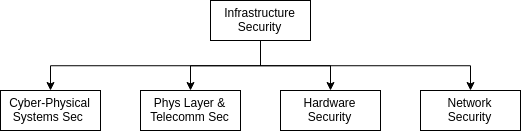
\includegraphics[width=.75\linewidth]{resource/img/ch_background/cybok_metrics/cybok_infra.png}
\end{mdframed}
\caption{Cybok: Infrastructure Domain Metrics
\label{fig:background:cybok_infra_metrics}}
\end{figure} 



Cyber-Physical Systems (CPS) includes SCADA and other control systems, vehicle networks, and IoT systems that fall outside the scope of this thesis but certainly have applicable security metrics associated with attack surface and information leakage. Similarly, most aspects of the other infrastructure components listed above are captured in the system and threat model and included in the Attack \& Defense security metrics. Types of security metrics applicable here but not listed in the surveys above might include supply chain vulnerabilities, weakness to eavesdropping or side channel attacks. 

\subsubsection{Software \& Platform Security Metrics}

\begin{figure}[ht]

\begin{mdframed}
\centering
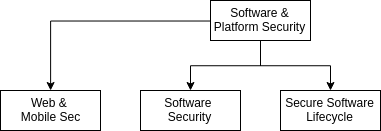
\includegraphics[width=.55\linewidth]{resource/img/ch_background/cybok_metrics/cybok_sw_platforms.png}
\end{mdframed}
\caption{Cybok: Software \& Platforms Domain Metrics
\label{fig:background:cybok_sw_metrics}}
\end{figure} 

Software security metrics were the focus of Morrison’s survey and apply here broadly. Typical applications of these type metrics derive from static analysis and test coverage. Of specific interest in the thesis is the remediation velocity, which measures the time between discovering a flaw in software and the time a fix has been merged into the code base.


\begin{figure}[ht]
\centering
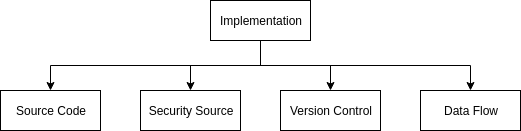
\includegraphics[width=.85\linewidth]{resource/img/ch_background/cybok_metrics/morrison_implementation.png}
\centering
\caption{Morrison’s Implementation Security metrics fall under SW\&P.
\label{fig:background:cybok_ad_vaugh_ttoa}}
\end{figure} 

% \subsubsection{Systems Security Metrics}

\subsubsection{Summary}

In the surveys summarized above there were over 500 distinct security metrics identified. The surveys each provided their own classification systems which were appropriate for the analysis they conducted, but none of these taxonomies generalize well to classify all types of security metrics. In this section we have described properties common to all metrics, identified overlaps in the various taxonomies, identified points of confusion between existing metric hierarchies, and described a suitable and intuitive system for classifying any current or future security metric. By using the Cybok as the underlying classification system we are also able to determine the distribution of metrics in each topic and identify areas of limited coverage which would benefit from future research.






